%!TEX root = index.tex
\chapter{Desenvolvimento}
\label{cha:desenvolvimento}

\section{Benchmark: Parcerias empresa-universidade} % (fold)
\label{sec:cases}

\subsection{TECNOPUC}

Os parques tecnológicos são um movimento de apoio à inovação e empreendedorismo que têm crescido muito nos últimos anos no Brasil. Eles se referem a aglomerações de empresas de base tecnológica, que podem ser pequenas ou não, articuladas a universidades e centros de P\&D, possibilitando sinergias decorrentes da proximidade entre os atores. \cite{parquestecnologicos} 

No Brasil há varios parques tecnológicos de destaque, como o Porto Digital em Recife, o Parque Tecnológico de São José dos Campos, o Parque Tecnológico da UFRJ e o Parque Científico e Tecnológico da PUC-RS (TECNOPUC). Dentre esse parques, a TECNOPUC se mostra um excelente caso de sucesso entre universidade e empresa, estimulando a pesquisa e a inovação por meio de uma ação simultânea entre academia, instituições privadas e governo, sob gestão da própria universidade.

O TECNOPUC possui um portfólio de empresas multissetorial, focado em quatro principais áreas definidas a partir da competência acadêmica da Universidade, envolvendo grupos de pesquisa científica e tecnológica, cursos de pós-graduação e à existência de demanda da sociedade. (Figura \ref{fig:tecnopuc})

\begin{figure}
\caption{Áreas de atuação do Tecnopuc}
\centerline{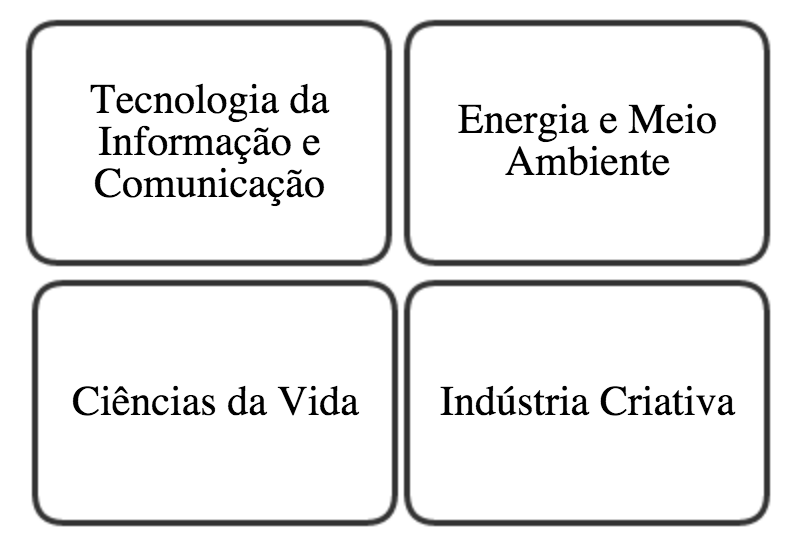
\includegraphics[scale=0.5]{img/tecnopuc}}
\label{fig:tecnopuc}
\caption* {Fonte: Adaptado do site do Tecnopuc}
\end{figure}

Atualmente, o TECNOPUC abriga 120 organizações, desde grandes companias de tecnologia como Samsung, Microsoft, Motorola e Dell até instituições financeiras como o HSBC. 

O TECNOPUC é um dos pilares do INOVAPUCRS - Rede de Inovação e Empreendedorismo da PUC-RS. Segundo \citeonline{tecnopuc}, o sucesso da iniciativa de inovação e empreendedorismo na universidade se deve à combinação do TECNOPUC com diversas outras estruturas de apoio:

\begin{description}
\item[AGT] - A Agência de Gestão Tecnológica facilita e articula a comunicação entre empresa e pesquisadores, identificando possíveis parcerias, acelerando a burocracia inerente a essas parcerias e captando recursos para viabilizar os projetos
\item[ETT] - O Escritório de Transferência de Tecnologia é responsável pelo estabelecimento e proteção das diretrizes de propriedade intelectual das pesquisas geradas em parcerias com empresas.
\item[IDEIA] - O Instituto de Pesquisa e Desenvolvimento possui uma infraestutura laboratorial para incubar projetos de diversas unidades acadêmicas.
\item[RAIAR] - A Incubadora Raiar é responsável por abrigar empresas derivadas de pesquisas estabelecidas na universidade por alunos, professores ou funcionários ou novos empreendimentos de empresas já estabelecidas no TECNOPUC.
\item[LABELO] - Os Laboratórios Especializados em Eletroeletrônica trabalha na prestação de serviços tecnológicos, apoiando o fortalecimento e a qualificação dos produtos para atender a regulamentos e normas internacionais.
\item[CI] - O Centro de Inovação é uma parceria feita com a Microsoft de forma a acelerar o uso de novas tecnologias e fomentar a indústria de software.
\item[NE] - O núcleo empreendedor tem como objetivo estimular o empreendedorismo na Universidade através de palestras, eventos e projetos que visam as oportunidades de mercado e a inovação.
\end{description}

O TECNOPUC tem como missão criar uma comunidade de pesquisa e inovação transdisciplinar por meio da colaboração entre academia, empresas e governo visando aumentar a competitividade dos seus atores e melhorar a qualidade de vida de suas comunidades. Ele se baseia nos seguintes objetivos:

\begin{itemize}
\item Atrair empresas de pesquisa e desenvolvimento (P,D e I) para trabalhar em parceria com a Universidade
\item Promover a criação e o desenvolvimento de novas empresas de base tecnológica
\item Atrair projetos de pesquisa e desenvolvimento tecnológico em geral
\item Estimular a inovação e a interação empresas-Universidade
\item Gerar uma sinergia positiva entre o meio acadêmico e o empresarial
\item Atuar de forma coordenada com as esferas governamentais, particularmente no âmbito do Projeto Porto Alegre Tecnópole
\end{itemize}

\subsection{\textit{Deutsche Telekom - T-labs}}

A \textit{Deutsche Telekom} (DT) é uma empresa de telecomuniçação Alemã e também a maior do setor em toda a União Européia. A compania possui um grande expertise na área de tecnologia da comunicação e tecnologia da informação, possuindo duas grandes subsidiárias: a operadora T-mobile e a consultoria de TI T-Systems, ambas com atuação global.

Por atuar em um segmento tão competitivo e totalmente dependente de inovações tecnológicas para gerar vantagem competitiva diante das outras empresas, a DT sempre apresentou muitas iniciativas e um forte investimento na área de P\&D. Através de uma dessas iniciativas surgiu a proposta dos Laboratórios \textit{Deutsche Telekom} (T-labs).

Os T-labs foram criados com o objetivo de pesquisar e desenvolver Tecnologia da Informação e Tecnologia da Comunicação de forma a permitir que novos negócios surjam e que operações já existentes sejam expandidas e acelerar o processo de inovação através da colaboração indústria e academia. \cite{dtlabs}

Para validar a real necessidade da DT em criar os laboratórios, foram levantadas as motivações apresentadas na tabela \ref{tab:motivacoes_dt}

\begin{table}[h]
\begin{center}
\caption{Fontes de Motivação para fundação dos T - Labs}
\label{tab:motivacoes_dt}
\begin{tabular}{>{\raggedright}p{0.25\linewidth}>{\raggedright\arraybackslash}p{0.55\linewidth}}
	\hline
    Importância & Indústria \\ 
    \hline \\
    \multirow{2}{*}{Razão Principal} 
    & Acesso à Inovação \\
    & Obter na fonte últimos avanços tecnológicos \\ \\
	\multirow{2}{*}{Alta relevância}
	& Constante atualização do \textit{know-how} \\
	& Canal de Recrutamento \\ \\
	\multirow{2}{*}{Média importância}
	& Diminuição de risco com pesquisas \\
	& Estabelecer projetos de longo prazo \\ \\
	\multirow{2}{*}{Baixa importância}
	& Diminuição de custos \\
	& Uso de laboratório \\ \\
\end{tabular}%
\caption* {Fonte: \citeonline{dtlabs}}
\end{center}
\end{table}

De forma geral, a DT buscava nos laboratórios uma porta de entrada para descobertas e inovações tecnológicas, além de possíveis novos funcionários e pesquisas de longo prazo.

Dadas as necessidades listadas, a DT sabia que o próximo passo para viabilizar o laboratório seria ultrapassar algumas barreiras existentes em parcerias universidade-empresa: barreiras culturais, institucionais e operacionais. \cite{barriers}

Em relação às barreiras culturais, foram definidos três principais pontos:
\begin{itemize}
\item Apenas são empregados pós doutorados com interesse em pesquisa orientada pela aplicação dos resultados da pesquisa
\item Políticas de publicação e de direito à propriedade intelectual foram bem definidas, com prazos e condições bem descritos
\item Compartilhamento de espaço físico e políticas internas tanto para o \textit{staff} acadêmico quanto da indústria.
\end{itemize}

Em relação às barreiras institucionais:
\begin{itemize}
\item Divisão de objetivos bem definida, com o \textit{staff} da academia voltado para a pesquisa estratégica, e o \textit{staff} da indústria voltado para atividades orientadas pelo desenvolvimento e inovação.
\item Resultados esperados pré definidos através de KPIs, de tal forma que cada área já sabe o que é esperado de si.
\item Separação e autonomia da gestão do laboratório por parte da empresa, de tal forma que mudanças corporativas na DT pouco interfiram no trabalho do laboratório.
\end{itemize}

Em relação às barreiras operacionais:
\begin{itemize}
\item Processos bem definidos 
\item Alinhamento entre áreas feito através da revisão trimestral de projetos e apresentações de progresso
\item Redução do princípio Não-Inventado-Aqui (NIA), no qual as corporações se recusam a usar soluções de terceiros para usar soluções desenvolvidas internamente.
\end{itemize}



\section{Identificação dos Stakeholders}
\label{sec:identificacao_stakeholders}

Ao longo da implementação do Ocean, foram definidos os seguintes stakeholders:

\begin{itemize}
\item PRO ( Chefia e COC [Zancul e Mesquita] e Pesquisa [Roberta])
\item Samsung (Selber, Conejo)
\item Alunos (CAEP, RD)
\item Usuários Externos ( Reinaldo [IGDA], Sakuda [Abragames], IoT)
\end{itemize}

\subsection{PRO}
\label{sec:con_pro}

Segundo \citeonline{jeeModels}, o ensino de engenharia pode ser dividido em 3 principais modelos: Acadêmico, Market-Driven e Integrativo.

\begin{table}[h]
\begin{center}
\caption{Modelos de ensino de engenharia}
\label{tab:modelos_ensino_tab}
{\def\arraystretch{2}\tabcolsep=10pt
\begin{tabular}{>{\raggedright}p{0.2\linewidth}>{\raggedright\arraybackslash}p{0.2\linewidth}>{\raggedright\arraybackslash}p{0.2\linewidth}>{\raggedright\arraybackslash}p{0.2\linewidth}}
\hline
     & Modelo Acadêmico & Modelo \textit{Market-Driven} & Modelo Integrativo \\ \hline
     Percepção de Engenharia & Ciência Aplicada & Inovação Tecnológica & Serviço Público \\
     Papel Social & Consultor, Especialista & Empreendedor, Gestor & Cidadão, Agente de Mudanças \\
     Perspectiva Institucional & Universidade Científica & Universidade Empreendedora & Universidade Ecológica  \\
	 Exemplos de Disciplinas & Cálculo, Estatística & Empreendedorismo, Desenvolvimento de Produto & Sustentabilidade, Problemas da Sociedade \\ \hline
\end{tabular}%
}
\caption* {Fonte: Adaptado de \citeonline{jeeModels}}
\end{center}
\end{table}

Dentro desse contexto, é possível observar uma grande sinergia entre o laboratório e o modelo \textit{Market-Driven}, pois o departamento pode o utilizar para auxiliar no desenvolvimento de engenheiros para estarem alinhados com as necessidades do mercado, sendo este representado por uma das empresas com maior tecnologia de ponto a nivel global.

\subsection{Samsung}
\label{sec:con_samsung}

De forma a incentivar a cultura, o esporte, o social e o desenvolvimento do país, foram criadas várias leis de incentivo para empresas a investirem nessas frentes a troca de uma renúncia fiscal.  Normalmente, o governo abre mão de parte dos impostos da empresa pois os mesmos serão destinados a outros projetos de benefício da sociedade. Do lado da empresa é extremamente positivo, pois esse incentivo pode ser usado tanto para reforçar a imagem da empresa quanto para gerar um retorno financeiro, fatos que não ocorreriam caso o mesmo investimento fosse aplicado em forma de impostos.

Entre essas leis encontra-se a Lei 8.248/91, conhecida como lei da informática, que foi sancionada em Outubro de 1991 pelo então presidente Fernando Collor. Dentro desta Lei o principal benefício é a redução da alíquota do IPI de 15\% para 3\% até 2029. Em contrapartida, a empresa beneficiada por essa Lei se compromete a investir até 4\% do faturamento de determinado segmento em Pesquisa e Desenvolvimento. É dentro do contexto dessa Lei que o Ocean retira grande parte dos recursos de subsidiação do laboratório. 

Ainda, por estar dentro da universidade, a Samsung têm acesso direto a especialistas com \textit{know how} restrito a poucas instituições no mundo e acesso a graduandos e pós-graduandos com potencial para futuros recrutamentos 

\subsection{Alunos}
\label{sec:con_alunos}

A presença de um laboratório como este também ajuda a fomentar a cultura de empreendedorismo dentro da universidade, pois deixa os alunos próximos ao desenvolvimento de software, uma das principais bases de criação de novas \textit{startups}, devido ao baixo custo de aprendizado e investimento e alto valor gerado no curto e médio prazo. Ainda, segundo \citeonline{entrepreneurship}, os estudantes de engenharia experienciam o empreendedorismo de 4 maneiras: 

\begin{enumerate}
\item Primeiro passo para o auto-aprendizado
\item Preparação para a vida no trabalho
\item Caminho para ser autônomo
\item Desenvolvimento de liderança e responsabilidade de um time
\end{enumerate}

\subsection{Usuários Externos}
\label{sec:con_usuarios}

Segundo a 27\textsuperscript{a} Pesquisa de Anual do uso de TI, realizada pela Fundação Getúlio Vargas (FGV), o número de smartphones em uso no Brasil gira atualmente em torno de 168 milhões de dispositivos. \cite{tifgv} Não obstante, além do alto número de smartphones, o Brasil também se mostra presente no mercado de outros dispositivos inteligentes, com previsão de movimentação de US\$4,1 bilhões no Brasil com IOT, segundo a assessoria de imprensa da IDC Brasil. \cite{idc}

É nesse cenário de alto crescimento do uso de novas tecnologias no Brasil que o mesmo se mostra como um grande mercado para produtos inerentes ao uso de dispositivos inteligentes, como aplicativos e games. Dentro desse contexto, jovens interessados pelo desenvolvimento desse mercado no país podem utilizar o Ocean para realizar diferentes cursos nessas áreas, desde aulas para iniciantes até cursos mais avançados.

Além do uso aplicado diretamente nessa área de dispositivos portáteis, a programação desenvolvida nessas atividades pode ser extendida para outras áreas de desenvolvimento, tornando os jovens mais capacitados para qualquer área tecnológica. Segundo a ONG Code.org, financiada por fundadores das maiores empresas de tecnologia do mundo como Mark Zuckerberg e Bill Gates, o número de empregos para programadores cresce exponencialmente, ao passo que o ensino de programação nas escolas não acompanha o mesmo ritmo, o que gerará uma falta de profissionais de TI em um futuro próximo. Juntamente a essa informação, o departamento de estatísticas de trabalho dos Estados Unidos (\textit{Bureau of Labor Statistics}) estima que o número de empregos para programadores dentro dos EUA diminuirá em até 8\%, pois mais profissionais deverão ser recrutados fora do país, devido ao baixo custo e a flexibilidade de trabalho remoto permitida pela programação. \cite{bls}

\section{Levantamento das necessidades} % (fold)
\label{sec:necessidades}

\section{Definição de processos} % (fold)
\label{sec:processos}

\section{Definição de indicadores} % (fold)
\label{sec:indicadores}